\chapter{面向大图的分层抽样算法}\label{chap:面向大图的分层抽样算法}

    \begin{algorithm}[!htbp]
        \small
        \caption{KSS 获取抽样结构$G_s$}\label{alg:k-ss-03}
        \begin{algorithmic}[1]
            \State \textbf{输入:} $V_{sup}$,$C_k$,$S_0,...,S_k$($X_1,...,X_M$),$T$,$p$
            \State \textbf{输出:} $G_s=(V_s,E_s)$
            \State \textbf{foreach} $v \in S_k$ \textbf{do}
            \State     \qquad \textbf{if} $\verb"Corevalues"(\verb"Neighbors"(v))==k$ \textbf{then} $V_{conn} \leftarrow v$
            \State     \qquad \textbf{else} $V_{disconn} \leftarrow v$
            \State \textbf{end }
            \State $i \leftarrow k-T$
            \State \textbf{while} $i > 0$ \textbf{do}
            \State     \qquad \textbf{foreach} $v \in S_i$ \textbf{do}
            \State     \qquad \qquad \textbf{if} $\verb"Shellvalues"(\verb"Neighbors"(v))\in[i-T,i]$ \textbf{then} $V_{conn} \leftarrow v$
            \State     \qquad \qquad  \textbf{else} $V_{disconn} \leftarrow v$
            \State     \qquad \textbf{end }
            \State     \qquad $V_s+=\verb"Sampling"(V_{conn},~k*p)$
            \State     \qquad $V_s+=\verb"Sampling"(V_{disconn},~(1-k)*p)$
            \State     \qquad $i \leftarrow i - T$
            \State \textbf{end while}
            \State $E_s \leftarrow \verb"getEdges"(V_s)$
            \State \textbf{return} $G_s=(V_s,E_s)$
        \end{algorithmic}
    \end{algorithm}


    \begin{figure}[!htbp]
        \begin{subfigure}[b]{0.31\textwidth}
          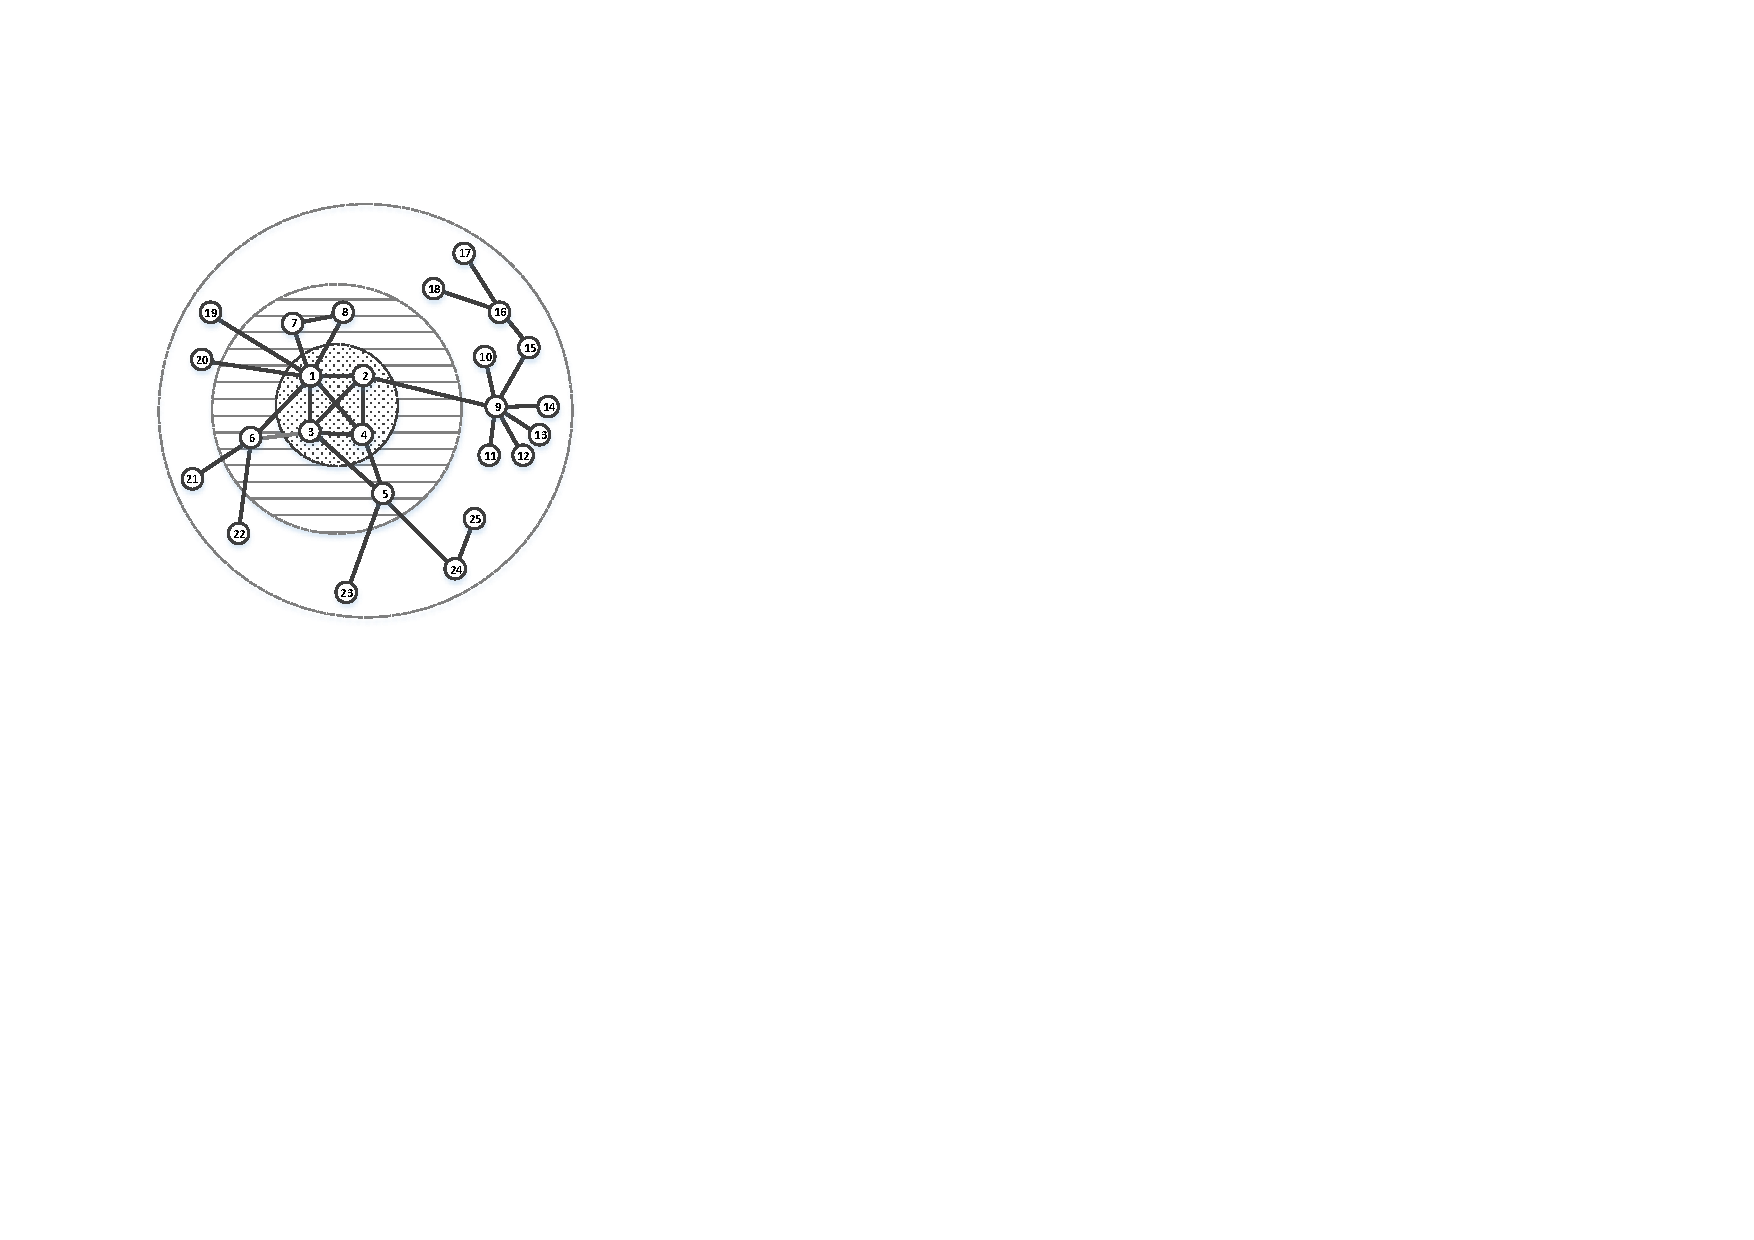
\includegraphics[width=\textwidth]{vis-4-study-a}
          \caption{}
          \label{fig:vis-4-study-a}
        \end{subfigure}
        ~
        \centering
        \begin{subfigure}[b]{0.31\textwidth}
          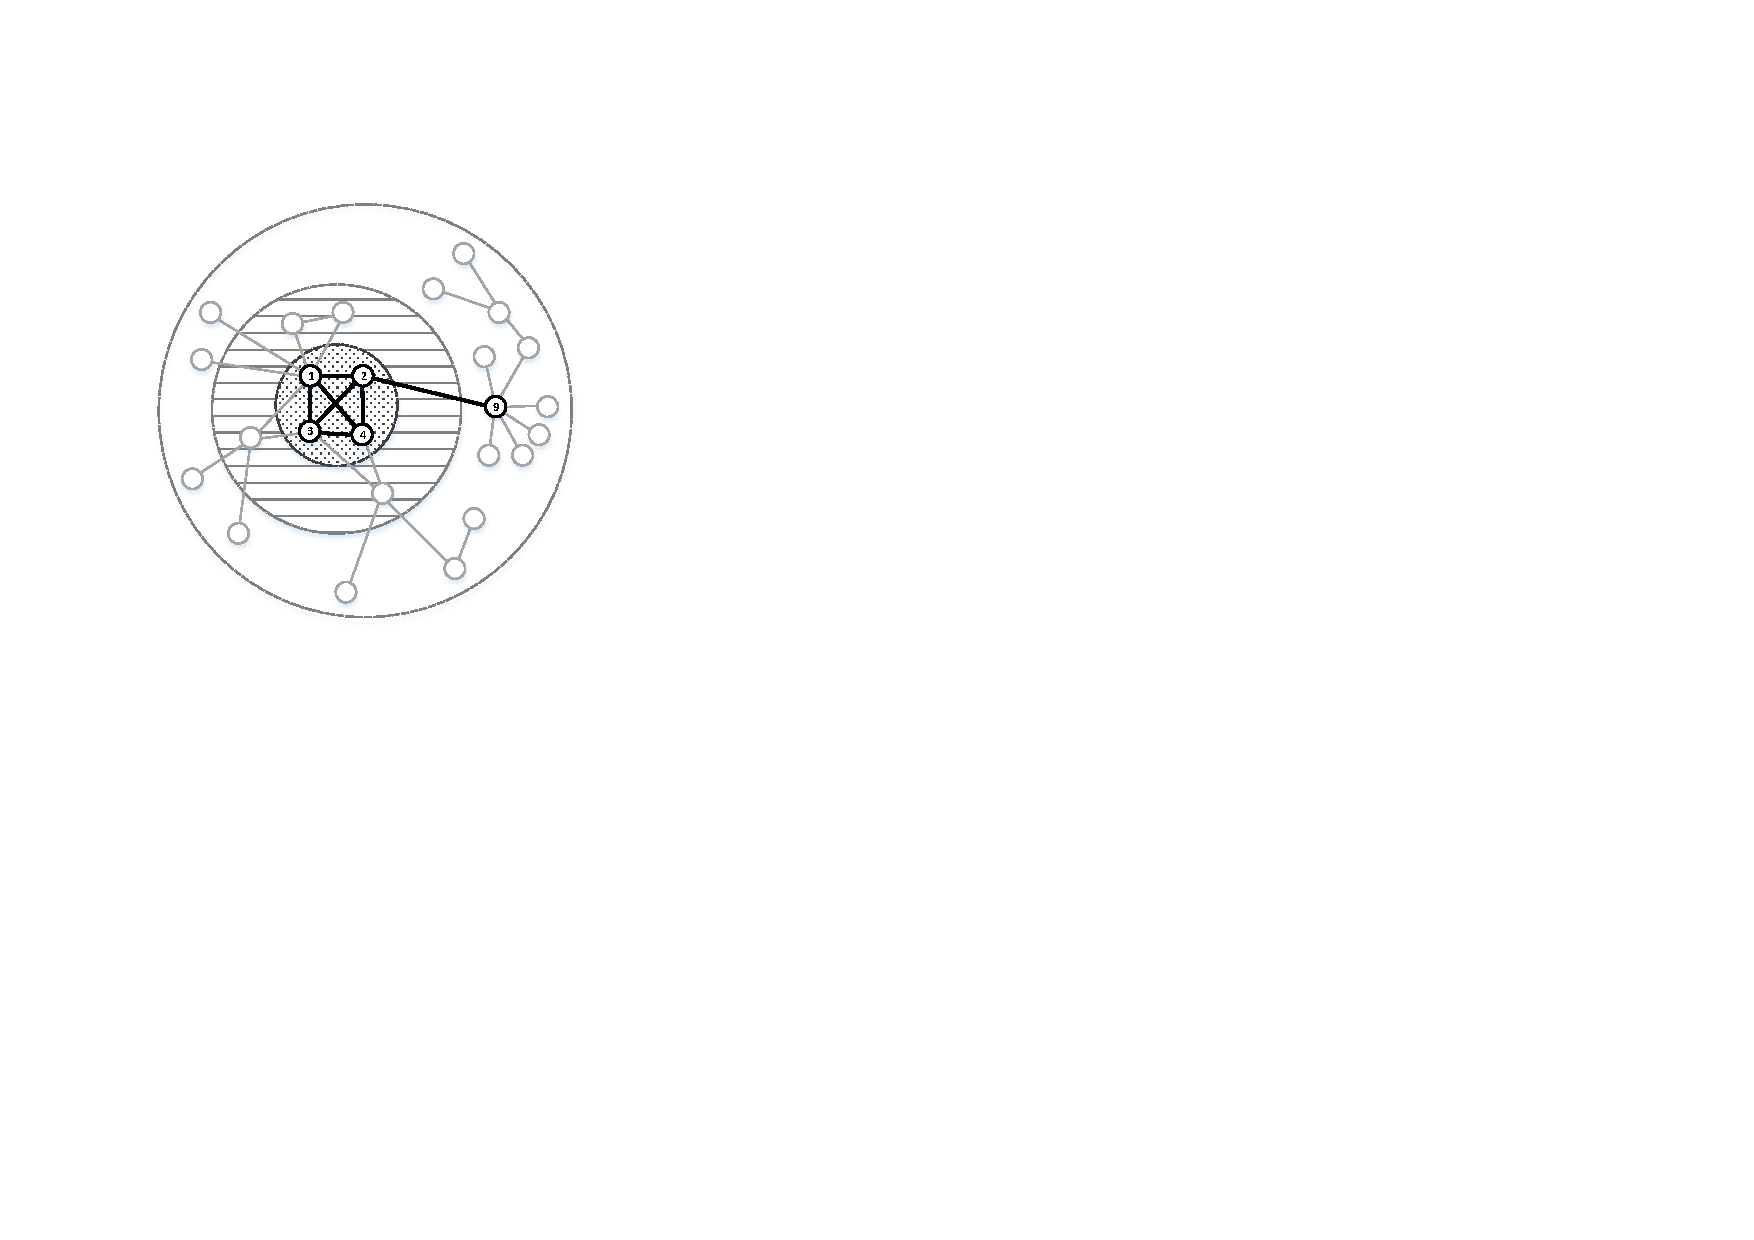
\includegraphics[width=\textwidth]{vis-4-study-b}
          \caption{}
          \label{fig:vis-4-study-b}
        \end{subfigure}%
        ~~%add desired spacing
        \centering
        \begin{subfigure}[b]{0.31\textwidth}
          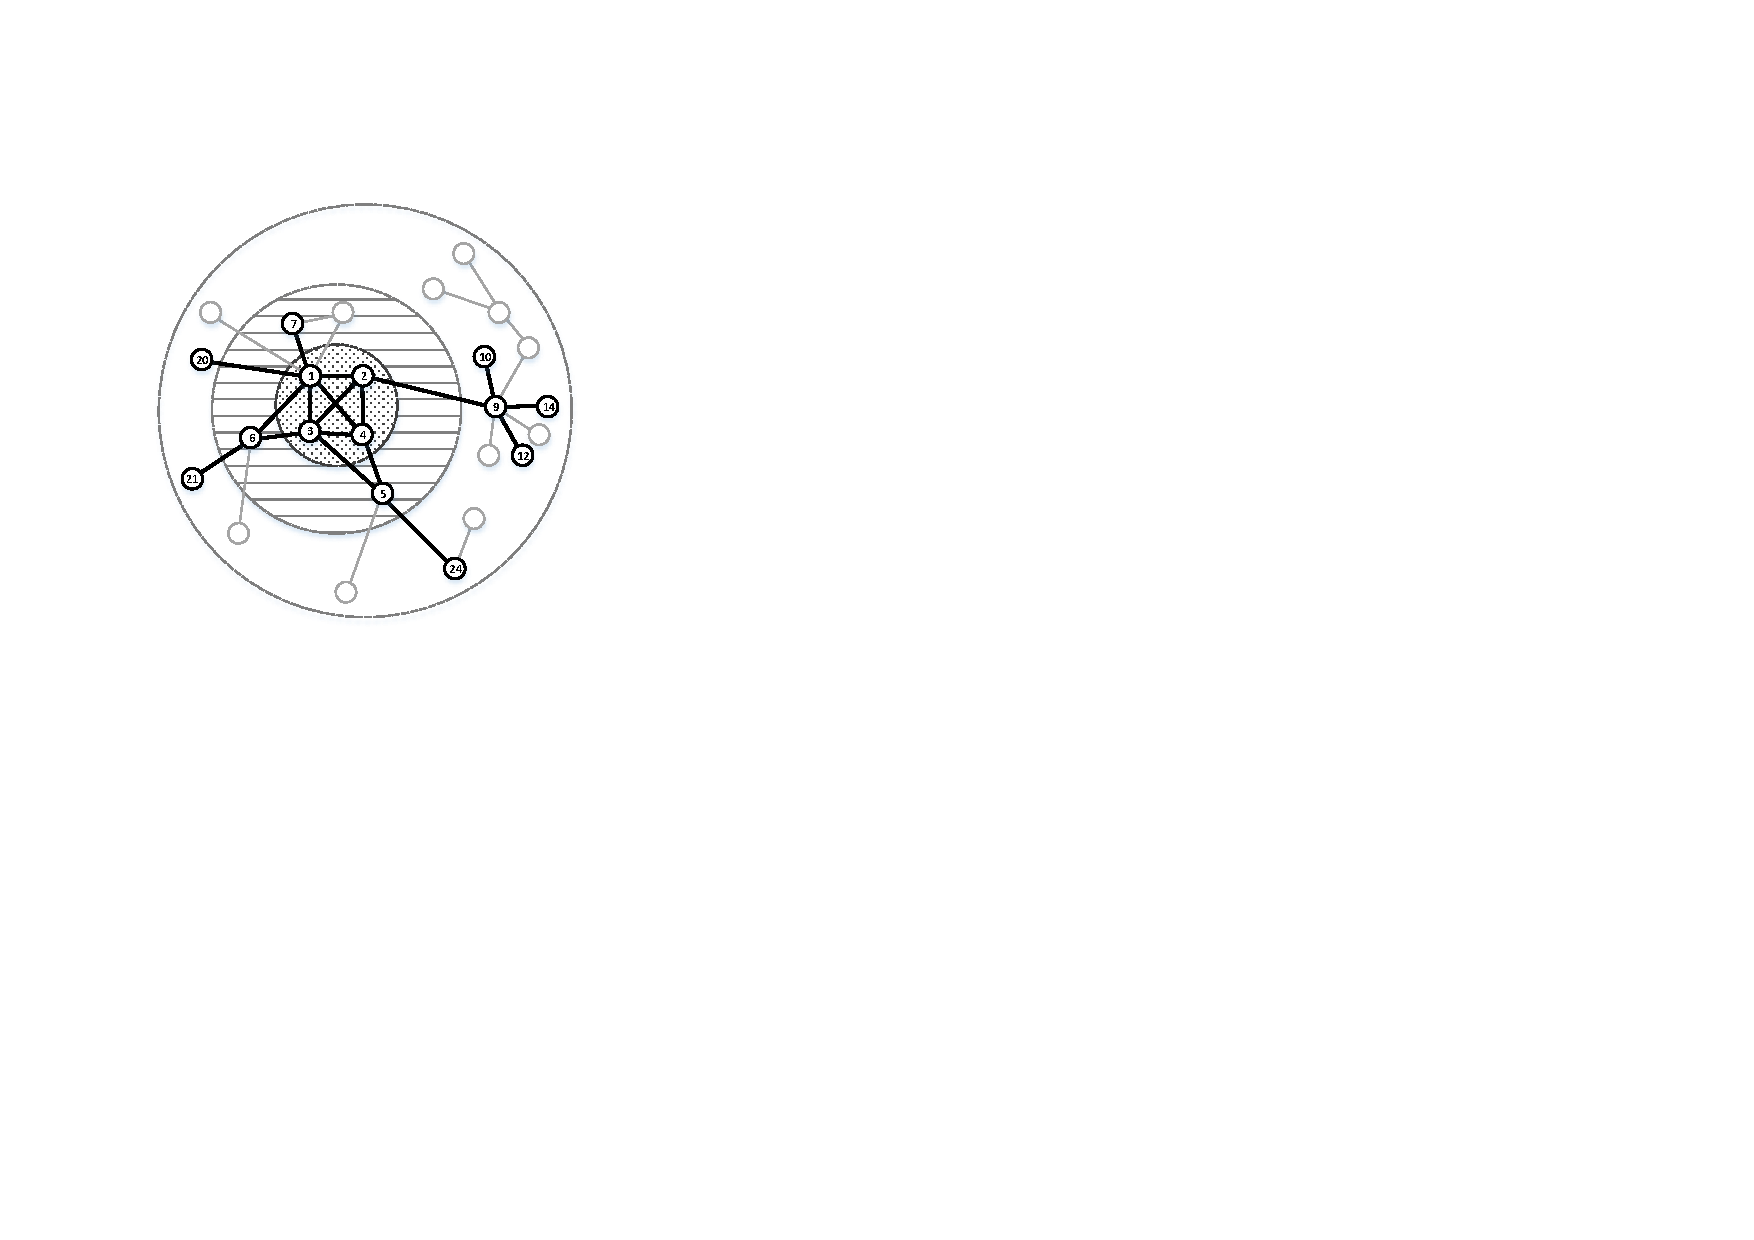
\includegraphics[width=\textwidth]{vis-4-study-c}
          \caption{}
          \label{fig:vis-4-study-c}
        \end{subfigure}%
        \bicaption{KSS抽样示例。(a) 示例结构,(b) 首层结构,(c) 最终结构。 }{Demo case of KSS. (a) Demo graph, (b) First layer structrue, (c) Final layer structure.}
        \label{fig:vis-4-study}
    \end{figure}


    \begin{table}[!htbp]
      \centering
      \bicaption{loc-Gowalla数据集的抽样效果。}{Sampling result of loc-Gowalla data set.}
      \fontsize{10}{10}\selectfont
      \setlength{\tabcolsep}{3mm}{
        \begin{tabular}{clllllll}
        \toprule
        \multicolumn{1}{l}{$Rate(\%)$} & $Algorithm$ & \multicolumn{1}{l}{$SM_d$} & \multicolumn{1}{l}{$V_{gc}^{'}$} & \multicolumn{1}{l}{$V_{cc}^{'}$} & \multicolumn{1}{l}{$V_{av}^{'}$} \\
        \midrule
        \multirow{5}[1]{*}{20} & RN    & 452.898 & 12.408 & 0.501 & 0.192 \\
              & RE    & 206.66 & 2.244 & 0.671 & 0.193 \\
              & SBS   & 239.564 & 1.035 & 0.59  & 1.398 \\
              & SS    & 237.636 & 0.712 & 0.113 & 2.756 \\
              & KSS   & 232.134 & 1.542 & 0.108 & 2.851 \\
        \midrule
        \multirow{5}[2]{*}{40} & RN    & 281.304 & 2.88  & 0.66  & 0.386 \\
              & RE    & 84.086 & 1.114 & 0.684 & 0.387 \\
              & SBS   & 207.437 & 0.869 & 0.567 & 1.446 \\
              & SS    & 167.298 & 0.612 & 0.175 & 2.017 \\
              & KSS   & 133.185 & 1.26  & 0.203 & 1.872 \\
        \midrule
        \multirow{5}[2]{*}{60} & RN    & 105.168 & 1.227 & 0.683 & 0.582 \\
              & RE    & 40.49 & 0.738 & 0.66  & 0.58 \\
              & SBS   & 180.316 & 0.807 & 0.574 & 1.423 \\
              & SS    & 166.767 & 0.516 & 0.295 & 1.451 \\
              & KSS   & 111.889 & 1.043 & 0.407 & 1.299 \\
        \bottomrule
        \end{tabular}%
        }
      \label{tab:3-testa-3}%
    \end{table}%




